\documentclass[12pt,a4paper]{article}
\usepackage[utf8]{vietnam}
\usepackage{amsmath,amssymb}
\usepackage{tabularx}
\usepackage{tikz}
\usetikzlibrary{calc,angles,quotes,arrows.meta,patterns}
\usepackage{xcolor}
\usepackage{enumitem}
\usepackage{fancyhdr}
\usepackage[top=1.2cm, bottom=1.2cm, left=1.5cm, right=1.5cm]{geometry}
\usepackage[loigiai]{ex_test}
\SAOPTN{widthSA=2.6,heightSA=0.62}

\setlength{\headheight}{15pt}
\setlength{\parskip}{0pt}

\pagestyle{fancy}
\fancyhf{}
\rhead{\textit{Môn Toán 6 -- Hướng dẫn giải Đề số 6}}
\lhead{\textit{Bộ đề ôn tập Giữa học kì I}}
\cfoot{\thepage}

\begin{document}

\begin{center}
  \textbf{\Large HƯỚNG DẪN GIẢI CHI TIẾT VÀ BẢNG ĐÁP ÁN}\\
  \textbf{\large ĐỀ ÔN TẬP GIỮA HỌC KỲ I -- ĐỀ SỐ 6}\\
  \textit{Môn: Toán 6 -- Năm học 2026 -- 2027}
\end{center}
\vspace{2mm}

% --- BẢNG ĐÁP ÁN TRẮC NGHIỆM TÓM TẮT ---
\noindent\textbf{\large A. BẢNG ĐÁP ÁN TRẮC NGHIỆM TỔNG HỢP}
\vspace{1.5mm}

\noindent\textbf{1. Phần I (Mỗi câu trả lời đúng được 0,25 điểm):}
\begin{center}
\begin{tabular}{|c|c|c|c|c|c|c|c|c|c|c|c|c|}
\hline
\textbf{Câu} & \textbf{1} & \textbf{2} & \textbf{3} & \textbf{4} & \textbf{5} & \textbf{6} & \textbf{7} & \textbf{8} & \textbf{9} & \textbf{10} & \textbf{11} & \textbf{12} \\
\hline
\textbf{Đ/A} & \textbf{B} & \textbf{A} & \textbf{B} & \textbf{A} & \textbf{D} & \textbf{B} & \textbf{B} & \textbf{A} & \textbf{B} & \textbf{A} & \textbf{C} & \textbf{C} \\
\hline
\end{tabular}
\end{center}
\vspace{1mm}

\noindent\textbf{2. Phần II (Đúng 1 ý: 0,1đ; 2 ý: 0,25đ; 3 ý: 0,5đ; 4 ý: 1,0đ):}
\begin{center}
\begin{tabular}{|c|c|c|c|c||c|c|c|c|c|}
\hline
\textbf{Câu} & \textbf{a)} & \textbf{b)} & \textbf{c)} & \textbf{d)} & \textbf{Câu} & \textbf{a)} & \textbf{b)} & \textbf{c)} & \textbf{d)} \\
\hline
\textbf{Câu 1} & \textbf{Đ} & \textbf{S} & \textbf{S} & \textbf{Đ} & \textbf{Câu 2} & \textbf{Đ} & \textbf{S} & \textbf{Đ} & \textbf{S} \\
\hline
\end{tabular}
\end{center}
\vspace{1mm}

\noindent\textbf{3. Phần III (Mỗi câu trả lời đúng được 1,0 điểm):}
\begin{center}
\begin{tabular}{|c|c|c|}
\hline
\textbf{Câu} & \textbf{Câu 1} & \textbf{Câu 2} \\
\hline
\textbf{Đáp án} & \textbf{3} & \textbf{48} \\
\hline
\end{tabular}
\end{center}
\vspace{3mm}

% --- B. LỜI GIẢI CHI TIẾT ---
\noindent\textbf{\large B. LỜI GIẢI CHI TIẾT CÁC CÂU HỎI}
\vspace{2mm}

\noindent\textbf{\large PHẦN I. CÂU TRẮC NGHIỆM NHIỀU PHƯƠNG ÁN LỰA CHỌN}
\vspace{1mm}
\begin{ex}
Khẳng định nào sau đây là sai?\\Trong hình vuông:
\choice
{Bốn cạnh bằng nhau}
{\True Hai đường chéo song song với nhau}
{Bốn góc ở các đỉnh là góc vuông}
{Hai cạnh đối song song}
\loigiai{
Hai đường chéo của hình vuông cắt nhau và vuông góc với nhau tại trung điểm của mỗi đường, chứ không song song với nhau. Do đó, khẳng định "Hai đường chéo song song với nhau" là sai.
}
\end{ex}

\begin{ex}
Cho tập hợp $A = \{0; 2; 4; a; b\}$. Khẳng định nào dưới đây sai?
\choice
{\True $5 \in A$}
{$a \in A$}
{$0 \in A$}
{$1 \notin A$}
\loigiai{
Số 5 không có trong tập hợp $A$, nên viết $5 \in A$ là khẳng định sai.
}
\end{ex}

\begin{ex}
Cho tập hợp $A = \{x \in \mathbb{N}^* \mid x \le 4\}$. Số nào dưới đây là phần tử của $A$?
\choice
{0}
{\True 4}
{5}
{6}
\loigiai{
Tập hợp các số tự nhiên khác 0 nhỏ hơn hoặc bằng 4 là $A = \{1; 2; 3; 4\}$. Do đó, 4 là một phần tử thuộc $A$.
}
\end{ex}

\begin{ex}
Với $a, m, n$ là các số tự nhiên, khẳng định nào sau đây đúng?
\choice
{\True $a^m : a^n = a^{m-n}$ ($a \ne 0, m \ge n$)}
{$a^m : a^n = a^{m+n}$ ($a \ne 0$)}
{$a^m : a^n = a^{m \cdot n}$ ($a \ne 0$)}
{$a^m : a^n = m - n$ ($a \ne 0$)}
\loigiai{
Công thức chia hai lũy thừa cùng cơ số là: $a^m : a^n = a^{m-n}$ (với $a \ne 0, m \ge n$).
}
\end{ex}

\begin{ex}
Kết quả của phép tính $256 - 98 + 137$ là:
\choice
{21}
{217}
{259}
{\True 295}
\loigiai{
Thực hiện phép tính từ trái sang phải: $256 - 98 + 137 = 158 + 137 = 295$.
}
\end{ex}

\begin{ex}
Đối với biểu thức không có dấu ngoặc và chỉ có các phép tính cộng, trừ, nhân, chia, lũy thừa, thì thứ tự thực hiện phép tính đúng là:
\choice
{Nhân và chia $\to$ Lũy thừa $\to$ Cộng và trừ}
{\True Lũy thừa $\to$ Nhân và chia $\to$ Cộng và trừ}
{Lũy thừa $\to$ Cộng và trừ $\to$ Nhân và chia}
{Cộng và trừ $\to$ Nhân và chia $\to$ Lũy thừa}
\loigiai{
Thứ tự thực hiện các phép tính chuẩn là: Lũy thừa $\to$ Nhân và chia $\to$ Cộng và trừ.
}
\end{ex}

\begin{ex}
Cho các số $3; 15; 29$. Số không là số nguyên tố trong các số đó là:
\choice
{3}
{\True 15}
{29}
{Cả 3 số trên}
\loigiai{
Số 15 ngoài ước 1 và 15 còn chia hết cho 3 và 5, nên 15 là hợp số.
}
\end{ex}

\begin{ex}
Trong các số sau, số nào chia hết cho 9?
\choice
{\True 144}
{249}
{379}
{199}
\loigiai{
Xét tổng các chữ số: số 144 có tổng các chữ số là $1 + 4 + 4 = 9 \ \vdots \ 9$. Các số còn lại có tổng chữ số không chia hết cho 9.
}
\end{ex}

\begin{ex}
Bạn An có ngày sinh là số nguyên tố lớn nhất nhỏ hơn 20, tháng sinh của bạn là số nguyên tố nhỏ nhất. Vậy bạn An có ngày và tháng sinh là:
\choice
{Ngày 19 tháng 3}
{\True Ngày 19 tháng 2}
{Ngày 7 tháng 2}
{Ngày 7 tháng 3}
\loigiai{
Số nguyên tố lớn nhất nhỏ hơn 20 là 19. Số nguyên tố nhỏ nhất là 2. Vậy bạn An sinh ngày 19 tháng 2.
}
\end{ex}

\begin{ex}
Hình nào dưới đây là tam giác đều?
\begin{center}
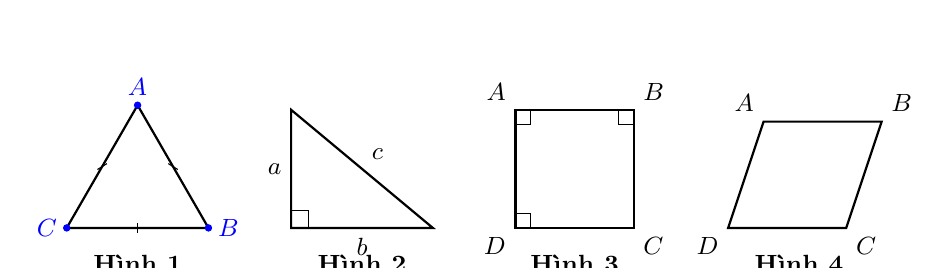
\begin{tikzpicture}[scale=0.75, font=\small]
  % Hinh 1: Tam giac deu ABC
  \begin{scope}[shift={(0,0)}]
    \coordinate (C) at (0,0);
    \coordinate (B) at (2.4,0);
    \coordinate (A) at (1.2, 2.078);
    \draw[thick] (A) -- (B) -- (C) -- cycle;
    \filldraw[blue] (A) circle (1.5pt) node[above] {$A$};
    \filldraw[blue] (B) circle (1.5pt) node[right] {$B$};
    \filldraw[blue] (C) circle (1.5pt) node[left] {$C$};
    \draw ($(A)!0.5!(B) + (-0.08,0.05)$) -- ($(A)!0.5!(B) + (0.08,-0.05)$);
    \draw ($(A)!0.5!(C) + (-0.08,-0.05)$) -- ($(A)!0.5!(C) + (0.08,0.05)$);
    \draw ($(B)!0.5!(C) + (0,-0.09)$) -- ($(B)!0.5!(C) + (0,0.09)$);
    \node at (1.2, -0.6) {\textbf{Hình 1}};
  \end{scope}
  % Hinh 2: Tam giac vuong
  \begin{scope}[shift={(3.8,0)}]
    \coordinate (V) at (0,0);
    \coordinate (X) at (2.4,0);
    \coordinate (Y) at (0,2);
    \draw[thick] (V) -- (X) -- (Y) -- cycle;
    \draw (0,0.3) -- (0.3,0.3) -- (0.3,0);
    \node[left] at (0,1) {$a$};
    \node[below] at (1.2,0) {$b$};
    \node[above right] at (1.2,1) {$c$};
    \node at (1.2, -0.6) {\textbf{Hình 2}};
  \end{scope}
  % Hinh 3: Hinh vuong ABCD
  \begin{scope}[shift={(7.6,0)}]
    \coordinate (D) at (0,0);
    \coordinate (C3) at (2,0);
    \coordinate (B3) at (2,2);
    \coordinate (A3) at (0,2);
    \draw[thick] (A3) -- (B3) -- (C3) -- (D) -- cycle;
    \draw (0,1.75) -- (0.25,1.75) -- (0.25,2);
    \draw (2,1.75) -- (1.75,1.75) -- (1.75,2);
    \draw (0,0.25) -- (0.25,0.25) -- (0.25,0);
    \node[above left] at (A3) {$A$};
    \node[above right] at (B3) {$B$};
    \node[below right] at (C3) {$C$};
    \node[below left] at (D) {$D$};
    \node at (1, -0.6) {\textbf{Hình 3}};
  \end{scope}
  % Hinh 4: Hinh binh hanh ABCD
  \begin{scope}[shift={(11.2,0)}]
    \coordinate (D4) at (0,0);
    \coordinate (C4) at (2,0);
    \coordinate (B4) at (2.6,1.8);
    \coordinate (A4) at (0.6,1.8);
    \draw[thick] (A4) -- (B4) -- (C4) -- (D4) -- cycle;
    \node[above left] at (A4) {$A$};
    \node[above right] at (B4) {$B$};
    \node[below right] at (C4) {$C$};
    \node[below left] at (D4) {$D$};
    \node at (1.2, -0.6) {\textbf{Hình 4}};
  \end{scope}
\end{tikzpicture}
\end{center}
\choice
{\True Hình 1}
{Hình 2}
{Hình 3}
{Hình 4}
\loigiai{
Quan sát hình vẽ thấy rằng Hình 1 có ký hiệu ba cạnh bằng nhau nên là tam giác đều.
}
\end{ex}

\begin{ex}
Mỗi góc của lục giác đều có số đo bằng:
\choice
{$90^\circ$}
{$180^\circ$}
{\True $120^\circ$}
{$60^\circ$}
\loigiai{
Lục giác đều có 6 góc ở các đỉnh bằng nhau, số đo mỗi góc bằng $120^\circ$.
}
\end{ex}

\begin{ex}
Một mảnh giấy hình chữ nhật có diện tích $120\text{ cm}^2$, độ dài một cạnh là $8\text{ cm}$. Chu vi của mảnh giấy là:
\choice
{$34\text{ cm}$}
{$40\text{ cm}$}
{\True $46\text{ cm}$}
{$54\text{ cm}$}
\loigiai{
Độ dài cạnh còn lại của mảnh giấy là: $120 : 8 = 15\text{ (cm)}$. Chu vi mảnh giấy là: $(15 + 8) \cdot 2 = 46\text{ (cm)}$.
}
\end{ex}


\setcounter{ex}{0}
\vspace{2mm}
\noindent\textbf{\large PHẦN II. CÂU TRẮC NGHIỆM ĐÚNG SAI}
\vspace{1mm}
\begin{ex}
Cho hình vuông $ABCD$ có cạnh bằng $4\text{ cm}$. Xét tính đúng/sai của các khẳng định sau:
\choiceTF
{\True $AB = BC = CD = DA = 4\text{ cm}$}
{$AB$ và $BD$ song song với nhau}
{Mỗi góc ở các đỉnh của hình vuông bằng nhau và bằng $60^\circ$}
{\True Vẽ cạnh $AB = 4\text{ cm}$. Dùng thước êke vẽ các đường vuông góc với $AB$ tại $A$ và $B$, sau đó lần lượt lấy các điểm $D, C$ trên các đường đó sao cho $AD = BC = 4\text{ cm}$. Nối $C$ với $D$ ta được hình vuông $ABCD$ có cạnh $4\text{ cm}$ như đã cho}
\loigiai{
\textbf{a)} Đúng. Hình vuông có 4 cạnh bằng nhau.

\textbf{b)} Sai. Cạnh $AB$ và đường chéo $BD$ cắt nhau tại đỉnh $B$, không song song với nhau.

\textbf{c)} Sai. Hình vuông có 4 góc ở các đỉnh bằng nhau và bằng $90^\circ$.

\textbf{d)} Đúng. Đây là các bước quy chuẩn để vẽ hình vuông khi biết độ dài cạnh bằng thước và êke.
}
\end{ex}

\begin{ex}
Cho tập hợp $A = \{x \in \mathbb{N} \mid 10 < x \le 15\}$. Xét tính đúng/sai của các khẳng định sau:
\choiceTF
{\True Tập hợp $A$ được viết dưới dạng liệt kê các phần tử là: $A = \{11; 12; 13; 14; 15\}$}
{Số 10 thuộc tập hợp $A$ (kí hiệu là $10 \in A$)}
{\True Trong tập hợp $A$, có đúng 2 phần tử là số nguyên tố}
{Tổng của phần tử lớn nhất và phần tử bé nhất trong tập hợp $A$ là một số chia hết cho 3}
\loigiai{
\textbf{a)} Đúng. Các số tự nhiên $x$ lớn hơn 10 và nhỏ hơn hoặc bằng 15 là 11, 12, 13, 14, 15.

\textbf{b)} Sai. Vì điều kiện là $x > 10$ nên $10 \notin A$.

\textbf{c)} Đúng. Trong tập hợp $A$, chỉ có 11 và 13 là số nguyên tố. Các số còn lại là hợp số.

\textbf{d)} Sai. Phần tử lớn nhất là 15, bé nhất là 11. Tổng: $15 + 11 = 26$. Vì tổng chữ số $2 + 6 = 8$ không chia hết cho 3 nên 26 không chia hết cho 3.
}
\end{ex}


\setcounter{ex}{0}
\vspace{2mm}
\noindent\textbf{\large PHẦN III. CÂU HỎI TRẢ LỜI NGẮN}
\vspace{1mm}
\begin{ex}
Tìm số tự nhiên $x$ thỏa mãn $2^x \cdot 4 = 32$. \shortans{3}
\loigiai{
Ta có: $4 = 2^2$ và $32 = 2^5$. Phương trình trở thành: $2^x \cdot 2^2 = 2^5 \Rightarrow 2^{x+2} = 2^5 \Rightarrow x + 2 = 5 \Rightarrow x = 3$.
}
\end{ex}

\begin{ex}
Một hình chữ nhật có chu vi bằng $28\text{ cm}$ và chiều dài bằng $8\text{ cm}$. Tính diện tích của hình chữ nhật đó (theo đơn vị $\text{cm}^2$). \shortans{48}
\loigiai{
Nửa chu vi của hình chữ nhật là: $28 : 2 = 14\text{ (cm)}$.\\Chiều rộng của hình chữ nhật là: $14 - 8 = 6\text{ (cm)}$.\\Diện tích hình chữ nhật là: $8 \times 6 = 48\text{ (cm}^2\text{)}$.
}
\end{ex}


\setcounter{ex}{0}
\vspace{2mm}
\noindent\textbf{\large PHẦN IV. TỰ LUẬN (BÀI TẬP VÀ BAREM ĐIỂM)}
\vspace{1mm}
\begin{ex} (1,5 điểm)
Thực hiện phép tính (Tính hợp lí nếu có thể):
\begin{enumerate}[label=\textbf{\alph*)}, leftmargin=0.8cm, itemsep=2pt]
\item (0,5 điểm) $12 \cdot 25 + 85 : 17 - 205$
\item (0,5 điểm) $5^2 \cdot 13 - 5^2 \cdot 3$
\item (0,5 điểm) $57 - [250 : (7 - 2)^2 - 3] \cdot 2025^0$
\end{enumerate}
\loigiai{
\textbf{a)} \textbf{[0,5 điểm]}\\ $12 \cdot 25 + 85 : 17 - 205 = 300 + 5 - 205 = 305 - 205 = 100$.

\textbf{b)} \textbf{[0,5 điểm]}\\ $5^2 \cdot 13 - 5^2 \cdot 3 = 25 \cdot (13 - 3) = 25 \cdot 10 = 250$.

\textbf{c)} \textbf{[0,5 điểm]}\\ $57 - [250 : 5^2 - 3] \cdot 1 = 57 - [250 : 25 - 3] = 57 - [10 - 3] = 57 - 7 = 50$.


}
\end{ex}
\vspace{2mm}

\begin{ex} (1,5 điểm)
Tìm số tự nhiên $x$, biết:
\begin{enumerate}[label=\textbf{\alph*)}, leftmargin=0.8cm, itemsep=2pt]
\item (0,5 điểm) $x + 12 = 45$
\item (0,5 điểm) $333 - x = 5^6 : 5^3$
\item (0,5 điểm) $(2x + 2)^3 = 12 \cdot 144$
\end{enumerate}
\loigiai{
\textbf{a)} \textbf{[0,5 điểm]}\\ $x = 45 - 12 \Rightarrow x = 33$.

\textbf{b)} \textbf{[0,5 điểm]}\\ $333 - x = 5^3 \Rightarrow 333 - x = 125 \Rightarrow x = 333 - 125 \Rightarrow x = 208$.

\textbf{c)} \textbf{[0,5 điểm]}\\ $(2x + 2)^3 = 12 \cdot 12^2 = 12^3 \Rightarrow 2x + 2 = 12 \Rightarrow 2x = 10 \Rightarrow x = 5$.


}
\end{ex}
\vspace{2mm}

\begin{ex} (1,5 điểm)
Kích thước chuẩn của sân bóng đá mini cho 5 người là sân hình chữ nhật có chiều dài tối thiểu $25\text{ m}$ và tối đa $42\text{ m}$, chiều rộng tối thiểu $15\text{ m}$ và tối đa $25\text{ m}$. Trường THCS A xây dựng sân bóng đá cỏ nhân tạo hình chữ nhật có chiều dài $30\text{ m}$, chiều rộng $20\text{ m}$.
\begin{enumerate}[label=\textbf{\alph*)}, leftmargin=0.8cm, itemsep=2pt]
\item (0,75 điểm) Vẽ minh họa sân bóng đá hình chữ nhật $ABCD$ có cạnh $AB = 3\text{ cm}$ và cạnh $BC = 2\text{ cm}$.
\item (0,75 điểm) Tính diện tích sân bóng đó.
\end{enumerate}
\loigiai{
\textbf{a)} \textbf{[0,75 điểm]}\\ \textbf{Cách vẽ hình chữ nhật $ABCD$ ($AB = 3\text{ cm}, BC = 2\text{ cm}$):}
\begin{itemize}[leftmargin=1.5cm, topsep=1pt, itemsep=1pt]
  \item Vẽ đoạn thẳng $AB = 3\text{ cm}$.
  \item Vẽ đường thẳng vuông góc với $AB$ tại $A$, trên đó lấy điểm $D$ sao cho $AD = 2\text{ cm}$.
  \item Vẽ đường thẳng vuông góc với $AB$ tại $B$, trên đó lấy điểm $C$ sao cho $BC = 2\text{ cm}$.
  \item Nối $C$ với $D$ ta được hình chữ nhật $ABCD$.
\end{itemize}
\begin{center}
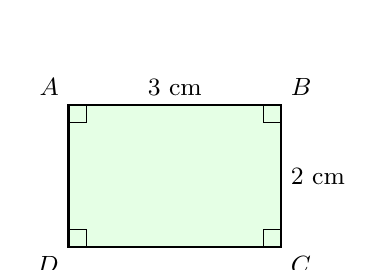
\begin{tikzpicture}[scale=0.9, font=\small]
  \coordinate (A) at (0,2);
  \coordinate (B) at (3,2);
  \coordinate (C) at (3,0);
  \coordinate (D) at (0,0);
  \draw[thick, fill=green!10] (A) -- (B) -- (C) -- (D) -- cycle;
  \draw (0,1.75) -- (0.25,1.75) -- (0.25,2);
  \draw (3,1.75) -- (2.75,1.75) -- (2.75,2);
  \draw (3,0.25) -- (2.75,0.25) -- (2.75,0);
  \draw (0,0.25) -- (0.25,0.25) -- (0.25,0);
  \node[above left] at (A) {$A$};
  \node[above right] at (B) {$B$};
  \node[below right] at (C) {$C$};
  \node[below left] at (D) {$D$};
  \node[above] at (1.5,2) {$3\text{ cm}$};
  \node[right] at (3,1) {$2\text{ cm}$};
\end{tikzpicture}
\end{center}

\textbf{b)} \textbf{[0,75 điểm]}\\ Diện tích sân bóng đá của trường THCS A là:\\$S = 30 \cdot 20 = 600\text{ (m}^2\text{)}$.


}
\end{ex}
\vspace{2mm}

\begin{ex} (0,5 điểm)
Một người bán 6 giỏ cam và xoài. Mỗi giỏ chỉ đựng hoặc cam hoặc xoài với số lượng sau: 34 quả, 39 quả, 40 quả, 41 quả, 42 quả, 46 quả. Sau khi bán một giỏ xoài thì số cam còn lại gấp 4 lần số xoài còn lại. Hãy cho biết giỏ nào đựng cam, giỏ nào đựng xoài?
\loigiai{
Tổng số quả trong 6 giỏ là:\\$34 + 39 + 40 + 41 + 42 + 46 = 242\text{ (quả)}$.\\Vì số cam còn lại gấp 4 lần số xoài còn lại nên tổng số quả còn lại chia hết cho $1 + 4 = 5$.\\Do 242 chia cho 5 dư 2 nên giỏ xoài đã bán phải chứa số quả chia cho 5 dư 2.\\Trong 6 giỏ đã cho, chỉ có số $42$ chia cho 5 dư 2 ($42 = 5 \cdot 8 + 2$). Do đó giỏ xoài đã bán là giỏ 42 quả.\\Tổng số quả còn lại là: $242 - 42 = 200\text{ (quả)}$.\\Số quả xoài còn lại là: $200 : 5 = 40\text{ (quả)}$.\\Vậy:\\-- Các giỏ đựng xoài gồm: giỏ 42 quả và giỏ 40 quả.\\-- Các giỏ đựng cam gồm: giỏ 34 quả, giỏ 39 quả, giỏ 41 quả và giỏ 46 quả.
}
\end{ex}
\vspace{2mm}


\begin{center}
\rule{4cm}{0.4pt}\\
\textit{--- HẾT ---}
\end{center}
\end{document}
